\documentclass[12pt]{article}

\usepackage{graphicx}
\usepackage{subcaption}
\usepackage{float}

\title{Parallelized Molecular Dynamics using Graphical Processing Units}
%\subtitle{APC 523}

\author{Nathan Mahynski \and George Khoury \and Carmeline Dsilva}


\begin{document}

\maketitle

\section{Introduction}

Due to the dramatic increase in computing power over the last thirty years, molecular dynamics simulations have become a remarkably fruitful tool for scientific discovery and engineering exploration.
%
These simulations allow us to screen potential drug compounds \cite{...}, explore protein folding dynamics \cite{...}, and develop new catalysts \cite{...}, all without running expensive and time-consuming experiments in a laboratory.
%
However, the requisite time and length scales for physically relevant simulations require some degree of parallelization to be computationally tractable on current computers.

At its core, molecular dynamics numerically integrates Newton's equation of motion ($force = mass \times acceleration$) forward in time.
%
Different numerical integration schemes result in different numerical accurracies for the simulations.
%
Standard molecular dynamics fixes the number of particles, volume, and total energy of the system.
%
However, one can introduce thermostats and barostats to the integration algorithm to fix the temperature and pressure of the system.

We implemented a software package to run molecular dynamics simulations in parallel.
%
The current version of the software implements the Lennard-Jones potential for interatomic interactions, a velocity-Verlet integrator, and a Nos\'{e}-Hoover thermostat; however, the software is sufficiently modular that other integration algorithms and pair potentials can easily be incorporated in later versions.
%
We chose to include the Lennard-Jone potenial because many of the standard force fields today are built on Lennard-Jones interactions.
%
For example, a commonly used model for water, the TIP3P water model \cite{jorgensen1983comparison}, is composed of Lennard-Jones interactions and an additional electorstatic term to account for water's polariazibiliy.
%
In addition, Lennard-Jones particles serve as a very good model for monotomic gases such as argon \cite{...}, crystals such as Iron \cite{...}, and condensed amporphous phases such as glasses \cite{...}.
%
The velocity-Verlet algorithm \cite{...} is accurrate to fourth order, ADD MORE.
%
The Nos\'{e}-Hoover thermostat is WHY IS THIS BETTER?

Because parallelization is essential for modern day molecular dynamics software, we implemented our software to run in parallel on both CPUs (with shared memory) and GPUs.
%
Our code is therefore fairly flexible and applicable to many different hardware architectures.

\section{Theory and Algorithms}

In the following section, we assume that our system of interest consists of $N$ particles.
%
We denote the position, velocity, and acceleration of particle $i$ as $\mathbf{r}_i$, $\mathbf{v}_i$, and $\mathbf{a}_i$, respectively. 
%
We denote the force on particle $i$ as $\mathbf{F}_i$.

In general, the algorithm for a molecular dynamics simulation is as follows:
\begin{enumerate}
\item Initialize particle positions $\mathbf{r}_i$ and velocities $\mathbf{v}_i$ within the simulation box.
\item  \label{itm:MD_start} Calculate the forces $\mathbf{F}_i$ on each particle.
\item \label{itm:MD_end} Integrate forward the positions and velocities of each particle for the chosen timestep $\Delta t$.
\item Repeat steps \ref{itm:MD_start}-\ref{itm:MD_end} for the chosen amount of simulation time.
\end{enumerate}

\subsection{Integrator} \label{subsec:integrator}

We implemented a velocity-Verlet integrator.
%
For fixed number of particles (N), volume of the system (V), and energy (E), we update the postions and velocities of each atom using the following equations
\begin{eqnarray}
\mathbf{r}_i (t + \Delta t)  & = & \mathbf{r}_i(t) + \mathbf{v}_i(t) \Delta t + \mathbf{a}_i(t) \frac{\Delta t^2}{2} \\
\mathbf{v}_i(t + \Delta t) & = & \mathbf{v}_i(t) + \left[\mathbf{a}_i(t) + \mathbf{a}_i(t + \Delta t) \right] \frac{\Delta t}{2}
\end{eqnarray}
where $\mathbf{a}_i = \mathbf{F}_i/m$.
%
The forces can be calculated from the potential energy function  and will be discussed further in subsection \ref{subsec:potential}.

Because $\mathbf{v}_i$ depends on both $\mathbf{a}_i(t)$ and $\mathbf{a}_i(t+\Delta t)$, the order of computations goes as follows 
\begin{enumerate}
\item Calculate $\mathbf{r}_i(t + \Delta t)$ from $\mathbf{r}_i(t)$, $\mathbf{v}_i(t)$, and $\mathbf{a}_i(t)$.
\item Calculate $\mathbf{a}_i(t + \Delta t)$ from $\mathbf{r}_i(t + \Delta t)$. 
\item Calculate $\mathbf{v}_i(t + \Delta t)$ from $\mathbf{v}_i(t)$, $\mathbf{a}_i(t)$, and $\mathbf{a}_i(t + \Delta t)$. 
\end{enumerate}

\subsection{Thermostats} \label{subsec:thermostat}
The equations in \ref{subsec:integrator} are only for NVE simulations.
%
If we are instead interested in fixing temperature (T) rather than energy (E), we must introduce the idea of a {\em thermostat} to our simulations.
%
The thermostat adjusts the velocities of the particles so that they (on average) maintain the desired temperature.

We implemented a Nos\'{e}-Hoover thermostat in our molecular dynamics software.
%
The Nos\'{e}-Hoover thermostat adjusts the particle velocities based on the target temperature of the system and the current kinetic energy of the system. 
%
The thermostat is governed by its own equation of motion given by the position ($\xi$), velocity ($\dot{\xi}$), and acceleration ($\ddot{\xi}$) of the thermostat.

Let $T_{set}$ be the desired temperature.
%
Then the acceleration of the thermostat is given by
\begin{equation}
\ddot{\xi} = \frac{1}{Q} \left[ \sum_{i=1}^{N} m_i v_i^2 - N_f k_B T_{set} \right]
\end{equation}

The equations of motion for the particles and the thermostat are
\begin{eqnarray}
r_i(t + \Delta t) &=& r_i(t) + v_i(t) \Delta t + \left[ a_i(t) - v_i(t)\dot{\xi}(t) \right] \frac{\Delta t^2}{2}\\
v_i(t + \Delta t) &=& v_i(t) + \left[ a_i(t) - v_i(t) \dot{\xi}(t) \right] \frac{\Delta t}{2} + \left[a_i(t + \Delta t)  - v_i(t + \Delta t) \dot{\xi}(t + \Delta t) \right] \frac{\Delta t}{2} \\
\xi(t + \Delta t) & = & \xi(t) + \dot{\xi}(t) \Delta t + \ddot{\xi}(t) \frac{\Delta t^2 }{2} \\
\dot{\xi}(t + \Delta t)  & = & \dot{\xi}(t) + \left[ \ddot{\xi}(t) + \ddot{\xi} (t + \Delta t)  \right] \frac{\Delta t}{2}
\end{eqnarray}

The Nos\'{e}-Hoover thermostat can be shown to be time-reversible. SHOW THIS!!

\subsection{Pair potentials} \label{subsec:potential}

We implemented a shifted Lennard-Jones pair potential in our molecular dynamics software.
%
In the shifted Lennard-Jones potential, the potential energy of interaction between two particles is a function of the interatomic distance $r = \|\mathbf{r}_i - \mathbf{r}_j \|$, and is given by 
\begin{equation}
U(r) = 4 \epsilon\left[ \left( \frac{\sigma}{r-\delta} \right)^{12} - \left( \frac{\sigma}{r-\delta} \right)^6 \right] + U_{shift}
\end{equation}
where $\epsilon$, $\sigma$, $\delta$, and $U_{shift}$ are adjustable parameters.
%
The total potential energy of the system is then given by
\begin{equation}
U_{tot} = \sum_{i=1}^{N} \sum_{j=1}^{i-1} U\left( \| r_i - r_j \| \right)
\end{equation}

The force on a particle $F_i$ is the gradient of the potential, $F_i = \nabla_i U_{tot}$.
%
It can be shown that 
\begin{equation}
F_{i, x} = \sum_{j \ne i} \frac{d U\left( \| r_i - r_j \| \right)}{d \| r_i - r_j \| } \frac{x_i - x_j}{\|r_i - r_j\|}.
\end{equation}

The potential energy and force calculations involve $\mathcal{O}(N^2)$ calculations, since each of the $N$ particles interacts with the remaining $N-1$ particles.
%
Therefore, the potential energy and force calculation are the portions that are typically parallelized in an MD code.

\subsection{Parallellization}

We implemented parallelization on CPUs and GPUs in our molecular dynamics software.
%
In both cases, the parallelization is implemented in the force calculation. 

On CPUs, we parallelized our code using OpenMP.
%
Therefore, our code can run in parallel on any shared memory cluster. 
%
On GPUs, we parallelized our code using CUDA.

\subsection{Neighbor lists}

\subsection{Testing}

We implemented Google Tests within our software.
%
We implemented the following tests:
	\begin{itemize}
	\item[\texttt{NumAtoms}] verifies that the system class stores the correct number of atoms
	\item[\texttt{KineticEnergy}] calculates the kinetic energy for a two-atom system, and verifies that it is correctly returned by the KinE() function
	\item[\texttt{PotentialEnergy}] calculates the potential energy for a two-atom system, and verifies that it is correctly returned by the PotE() function
	\item[\texttt{ChangeBox}] changes the length of the simulation box and verifies that the box is correctly changed in the system definition
	\item[\texttt{PBC}] computes the distance between two particles using the minimum image convention and verifies that it is correctly computed for different scenarios (out of box, inside box, etc.)
	\end{itemize}
\section{Code Structure}

The software is implemented in C++.
%
The class structure is as follows
\begin{description}

\item[\texttt{common.h}] This class implements the error catching functions.

\item[\texttt{cudaHelper.h}] This function implements the cuda code for paralleization on GPUs.

\item[\texttt{cellList.cpp}] This class controls the cell lists (for parallelization on CPU) or neighbor lists (for parallelization on GPUs). 

\item[\texttt{dataTypes.h}] This function implements the custom structures, such as the atom struct, which stores the position, velocity, and acceleration of an atom.
	
\item[\texttt{integrator.cpp}] This class is a ``virtual'' class (maybe????)

\item[\texttt{nve.cpp}] This class implements the velocity-Verlet integration scheme for an NVE simulation.

\item[\texttt{nvt.cpp}] This class implements the velocity-Verlet integration scheme with a Nos\'{e}-Hoover thermostat for an NVT simulation.

\item[\texttt{potential.cpp}] The potential class implements the force and potential energy calculations for the standard Lennard-Jones potential. 
%
This class can be expanded to include other potential energy functions.

\item[\texttt{system.cpp}] This class stores all of the parameters relevant to the simulation system, such as the box size, potential energy function, and the number of atoms. 

\item[\texttt{utils.cpp}] This class implements the necessary ``helper'' functions for the simulation, such as the distance calculation with periodic boundary conditions using the minimum image convention.

\item[\texttt{main.cpp}]

\item[\texttt{unittests.cpp}] This file implements Google Tests for our software. 
%
We used a test fixture to initialize the same system construct for multiple tests.

\end{description}

\section{Results}

\subsection{Scaling studies}

\subsection{Benchmarking}

\subsection{Validation against literature values}

We validated our code against LAMMPS \cite{plimpton1995fast} (http://lammps.sandia.gov), an existing commercial molecular dynamics software.
%
We simulated a system of 4000 Lennard-Jones particles at a reduced temperature $T=0.71$. 
%
We used a cubic box with edge length $L=16.796$, so that the reduced density of the system $\rho = 0.8442$. 
%
We used a timestep $\Delta t=0.005$, and simulated for $10,000$ timesteps.


We compared the temperature, potential energy, total energy, and radial distribution function for the two simulations. 
%
The results are shown in Figure \ref{fig:lmp_compare}. 
% 
There is excellent agreement between our software (CBEMD) and the LAMMPS results. 

\begin{table}
	\begin{tabular}{| r | c | c |}
		\hline
		 & CBEMD & LAMMPS \\
		 \hline
		 T & 0.7104 & 0.7112 \\
		 \hline
		 Potential energy / atom & -5.6532 & -5.6594 \\
		 \hline
		 Total energy / atom & -4.5879 & -4.5929 \\
		 \hline
	\end{tabular}
	\caption{Comparison of average thermodynamic quantities for CBEMD and LAMMPS simulations.}
	\label{table:lmp_compare}
\end{table}
		 
\begin{figure}[H]
	\begin{subfigure}{0.5\textwidth}
	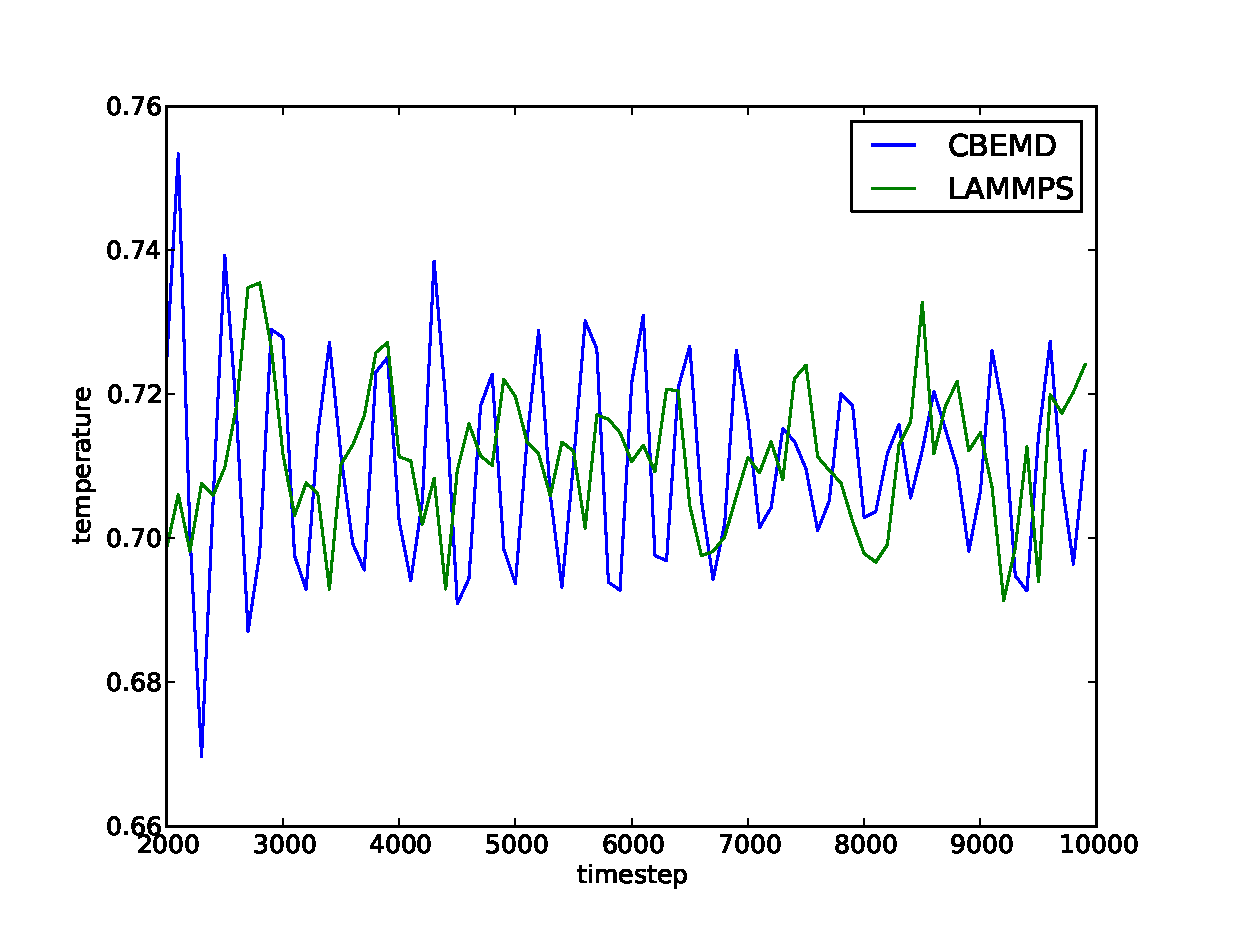
\includegraphics[width=\textwidth]{T_compare}
	\caption{}
	\end{subfigure}
	\begin{subfigure}{0.5\textwidth}
	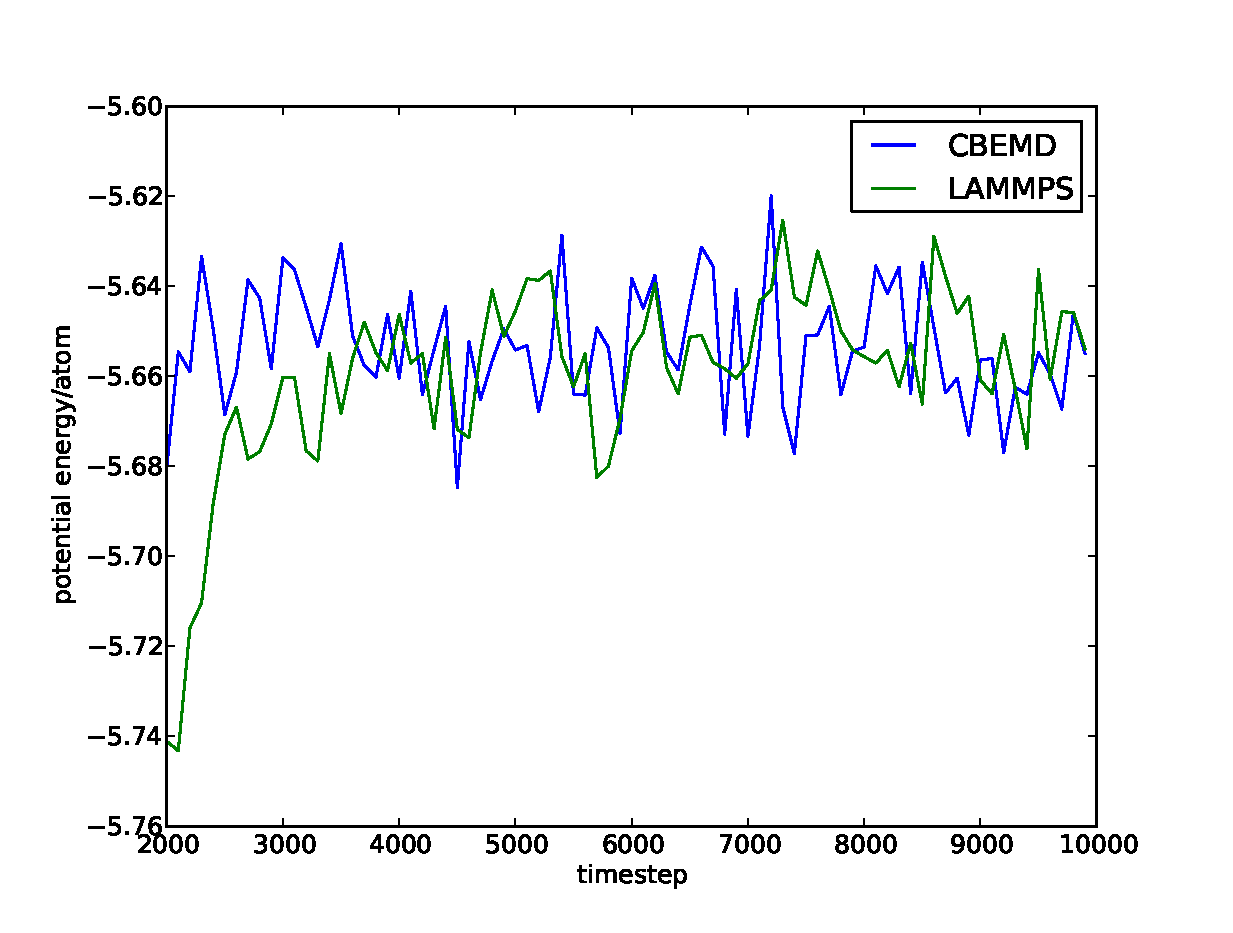
\includegraphics[width=\textwidth]{PE_compare}
	\caption{}
	\end{subfigure}
	\begin{subfigure}{0.5\textwidth}
	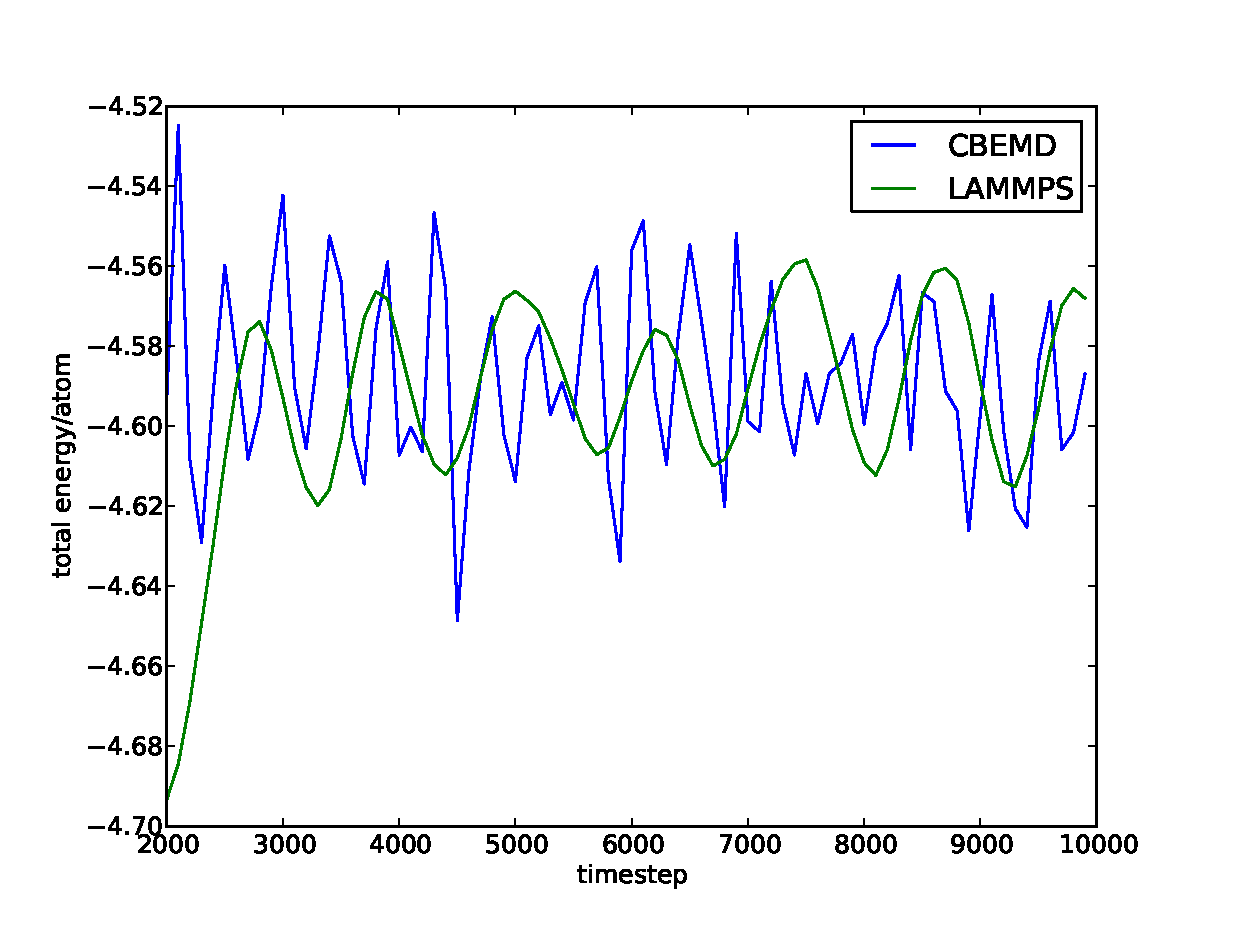
\includegraphics[width=\textwidth]{E_compare}
	\caption{}
	\end{subfigure}
	\begin{subfigure}{0.5\textwidth}
	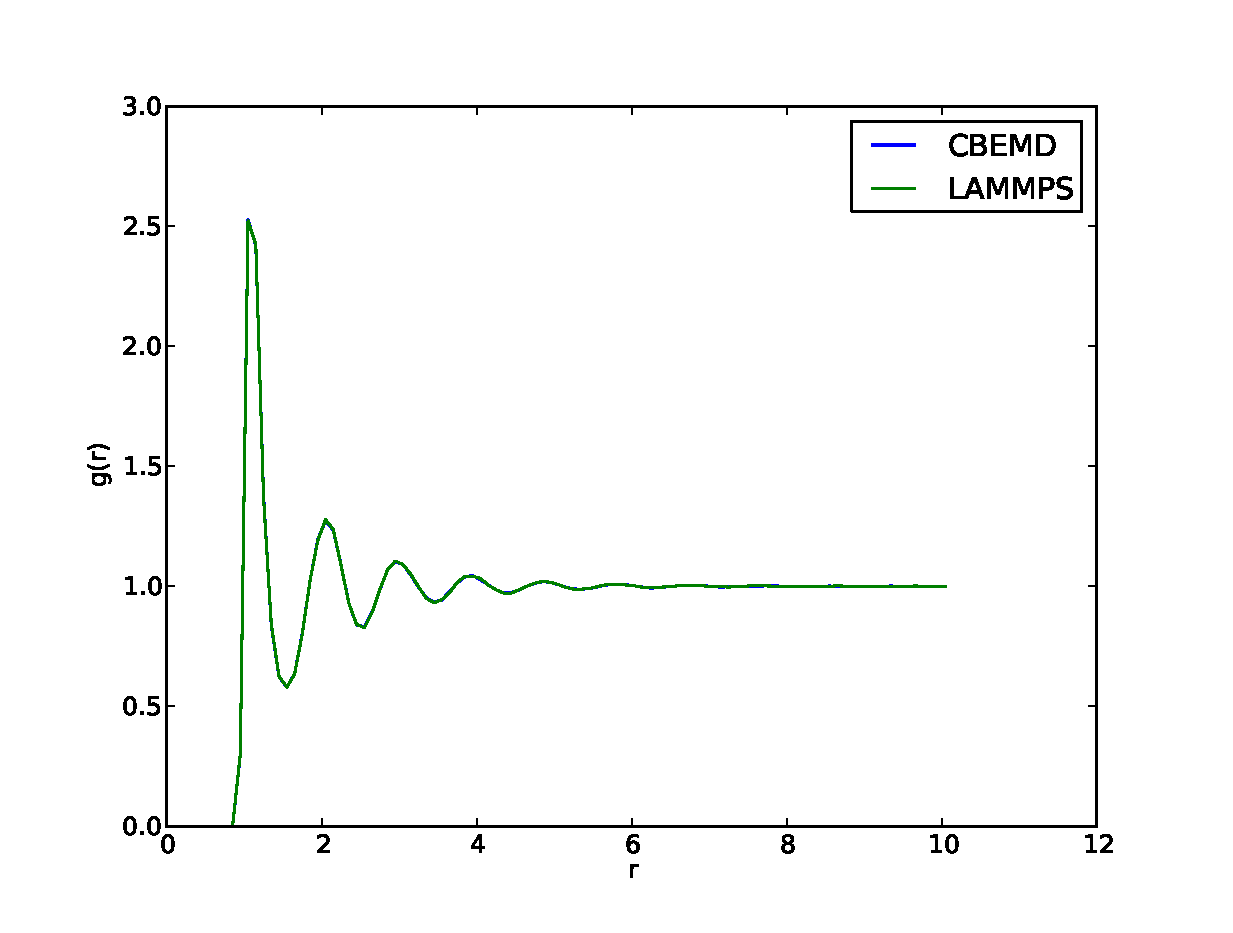
\includegraphics[width=\textwidth]{gr_compare}
	\caption{}
	\end{subfigure}
	\caption{Comparison between CBEMD simulation and LAMMPS simulation for 4000 Lennard Jones particles at $T=0.71$ and $\rho=0.8442$. (a) Comparison of temperature over time. (b) Comparison of potential energy/atom over time. (c) Comparison of total energy/atom over time. (d) Comparison of radial distribution functions. }
	\label{fig:lmp_compare}
\end{figure}
\section{Conclusions and Future Work}

\end{document}
